\documentclass[12pt,titlepage,french]{article}
\usepackage{babel}
\usepackage{graphicx}
\usepackage[margin=2.5cm]{geometry}
\usepackage{tabularx}
\usepackage[hidelinks]{hyperref}

\usepackage[utf8]{inputenc}
\usepackage[T1]{fontenc}
\pagestyle{plain}

\usepackage{booktabs,makecell,tabu}
\renewcommand\theadfont{\bfseries}

\linespread{1.5}

\begin{document}

\begin{titlepage}
\newcommand{\HRule}{\rule{\linewidth}{0.5mm}}
\center

  
\includegraphics[width=0.45\textwidth]{../ressources/img_logos/logo_polytech.png}\\[1cm]

  
\includegraphics[width=0.45\textwidth]{../ressources/img_logos/logo_taglabs.png}


\HRule \\[0.4cm]
{ \huge \bfseries Cahier des charges \\[0.15cm] }
Classification colorimétrique de nuages de points 3D
\HRule \\[1.5cm]
Ronan Collier,
Mathieu Letrone,
Tri-Thien Truong
\\[1cm]
\today \\ [1cm]
Version 1.1
\end{titlepage}

\tableofcontents % table des matières
\newpage
\listoffigures  % table des figures
\newpage

\section{Introduction}

\subsection*{Remerciements}

Nous tenons avant tout à remercier l'entreprise TagLabs, et plus particulièrement M. Yan KOCH, pour sa disponibilité et de sa confiance pour l'élaboration de ce projet.

Nous remercions également notre tuteur académique, M. Nicolas NORMAND, pour son temps accordé sur ce projet.

\subsection*{Contexte général du projet dans l'entreprise}

Taglabs est une jeune entreprise créée il y a deux ans par Yan Koch. L’entreprise s’inscrit dans le domaine de la modélisation 3D d’ouvrages. Ils proposent la modélisation et l’exploitation de nuages de points. Toutefois, ils travaillent surtout en interne sur un logiciel « ScanSap », le but de ce logiciel est d’exploiter les nuages de points 3D avec efficacité et simplicité inégalées.

Voulant continuer leur développement dans ce domaine encore nouveau, l'entreprise cherche maintenant à améliorer leurs outils, afin de compléter l'exploitation des nuages de points. L'ensemble de ces fonctionnalités permettent à leurs clients de pouvoir analyser un environnement en numérique, à un instant précis (qui sera sous la forme d'un scan de nuages de points). Par exemple, une entreprise peut avoir le besoin d'avoir un scan d'une de leur usine, afin d'analyser le positionnement de leurs machines, les potentielles fuites au niveau des tuyaux, etc.

L'équipe qui sera à la charge de ce projet est composée de trois étudiants en informatique à Polytech Nantes. Dans le cadre de la quatrième année dans la formation d'ingénieur informatique, nous devons réaliser un projet transversal avec une entreprise.

\subsection*{Présentation des parties prenantes du projet}

\subsubsection*{Maître d'ouvrage (MOA)}

Le MOA, ou \textbf{maître d'ouvrage}, est la partie cliente, elle représente l'entreprise formulant le besoin.
Elle va être chargée de valider les différentes itérations de la solution au fur et à mesure du projet.\\


\noindent\begin{tabu} to \textwidth {X[c]X[c]X[c]X[c]}\toprule
   \thead{Qui}&\thead{Rôle}&        \thead{Mail}&\thead{Mobile}\\\toprule
      Yan Koch&   Président&  yankoch@taglabs.fr&    0660239733\\\midrule
Robin Kervadec&   Ingénieur&rkervadec@taglabs.fr&    0619656021\\\bottomrule
\end{tabu}

\subsubsection*{Maître d'œuvre (MOE)}

Le MOE, ou \textbf{maître d'œuvre}, correspond au groupe responsable de la conception de la solution.
Le MOE dispose du choix des moyens techniques.
Dans le cadre de notre projet, la partie MOE est confondue avec l'équipe de développement, étant donné qu'elle est responsable à la fois de la conception et du développement.\\

\noindent\begin{tabu} to \textwidth {X[c2]X[c]X[c3]X[c]}\toprule
     \thead{Qui}&\thead{Rôle}&                       \thead{Mail}&\thead{Mobile}\\\toprule
Tri-thien Truong& Chef de projet&tri-thien.truong@etu.univ-nantes.fr&    0631193663\\\midrule
   Ronan Collier& Développeur&   ronan.collier@etu.univ-nantes.fr&    0666847162\\\midrule
 Mathieu Letrone& Développeur& mathieu.letrone@etu.univ-nantes.fr&    0789662916\\\bottomrule
\end{tabu}


\subsubsection*{Tuteur}

Le tuteur est l'encadrant du projet. Il veille à la conformité du projet avec les attentes du corps enseignant.
Il constitue une source de conseils pour le MOE, s'assure que le projet se déroule correctement entre le MOE et MOA, mais est aussi capable de lui appliquer des contraintes techniques.\\

\noindent\begin{tabu} to \textwidth {X[c2]X[c2]X[c3]X[c]}\toprule
     \thead{Qui}&\thead{Rôle}&                       \thead{Mail}&\thead{Mobile}\\\toprule
Nicolas Normand& Enseignant chercheur&Nicolas.Normand@univ-nantes.fr&    0240683207\\\bottomrule
\end{tabu}


\section{Modèle du domaine}

Cette partie va permettre de mieux représenter le projet vers une modélisation objet. Elle le décrit dans son ensemble via l'identification des entités ou concepts du domaine, et des associations entre ces derniers. \\

La solution devra permettre d’isoler, classifier un élément dans le nuage de points pour une meilleure visibilité et compréhension. Pour cela, la classification se basera selon la plage de couleur.\\

\begin{itemize}
        \item  S'il est déjà en couleur : on applique le filtre de plage colorimétrique pour isoler les éléments (Exemple: isoler les tubes proches du blanc).\par

        \item  S'il est en intensité de gris, on passe d'abord par de la fausse couleur, étape qui permet à l'utilisateur de mieux percevoir le nuage, puis on applique le filtre par plage colorimétrique.\\ \par
\end{itemize}

\begin{figure} [!hbtp]
\begin{minipage}[c]{0.60\linewidth}
La figure~\ref{Modèle du domaine} permet de résumer le modèle du domaine. Pour qu'un utilisateur classifie son élément dans un nuage de points donné, il devra segmenter ce dernier pour récupérer uniquement les éléments voulus. Il devra donc choisir une certaine couleur, représentée par les couleurs rouge, vert, bleu. Un nuage contient un grand nombre de points, qui ont pour caractéristique les coordonnées x, y, z (en trois dimensions). Chacun de ces points devront avoir une couleur.
\end{minipage} \hfill
\begin{minipage}[c]{0.40\linewidth}
    \centering
    \caption{Modèle du domaine}
    \label{Modèle du domaine}
    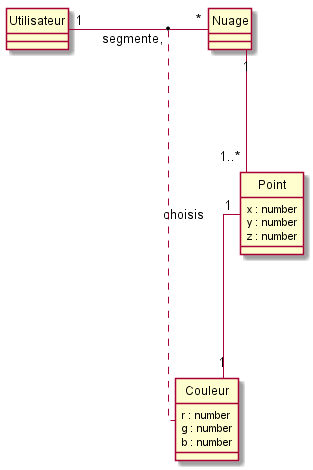
\includegraphics[scale=0.60]{img_diagrammes/modele_domaine.png}
    \end{minipage}
\end{figure}

\break
\section{Besoins fonctionnels}

Cette section concerne les besoins fonctionnels du projet.
Il s'agit des besoins du client auquel la solution se doit de répondre.

\subsection*{Utilisateur}
L'outil que nous développerons sera utilisé par les utilisateurs de "ScanSap", qui sont les clients de l'entreprise, mais aussi les membres de l'entreprise TagLabs.

\subsection*{Priorisation des tâches}

Afin de pouvoir définir la priorité des tâches et ainsi mettre en valeur leur importance, nous utiliserons la méthode MoSCoW. Cette méthode consiste à classifier les tâches selon 4 catégories :

\begin{itemize}
    \item \textbf{Must have} : Indispensables. Ils devront être traités en priorité.
    \item \textbf{Should have} : Importants. Ces tâches seront réalisables si tous les "Must have" auront été traité, et s'il reste du temps.
    \item \textbf{Could have} : Exigences additionnelles de confort. Cela pourra être intéressant de les avoir, mais peuvent être retirés des priorités s'il le faut.
    \item \textbf{Won't have} : Ils sont exclus de ce projet mais reste à côté pour une intégration future.
\end{itemize}

\subsection*{Description des besoins fonctionnels}

\noindent\begin{tabu} to \textwidth {p{0.15\textwidth}X[c2]X[c3]X[c3]}\toprule
     \thead{MoSCoW}&\thead{Fonctions}&\thead{Critères}&\thead{Flexibilité}\\\toprule
Must have
& Lire un fichier de données contenant un nuage de points
& Le nuage doit être visible à l'écran. La solution doit pouvoir lire un fichier au format ASCII. Elle doit reconnaître le format XYZ + RGB + intensité
& Visibilité complète du nuage de points donné. L'extension du fichier ainsi que l'ordre des points et des données de ces points sont laissés libre.\\\midrule
Must have
& Réaliser de la fausse couleur sur un nuage de points en intensité de gris
& Affichage dans la lecture du scan
& La couleur qui sera affichée devra correspondre à la couleur voulue avec une marge d'intensité de 5\%\\\midrule
Must have
& Exporter le nuage de points.
& Le nuage devra garder les modifications effectuées
& L'extension du fichier ainsi que l'ordre des points et des données de ces points est laissé libre.\\\midrule
Must have
& Isoler un élément dans un nuage de points donné, selon sa plage de couleur, son voisinage
& Les points isolés doivent appartenir à la plage de couleur désirée.
Les points appartenant à l'élément ciblé, mais de teintes différentes doivent également extraits (ombrages, réflexion, ...).
& Tolérance : plage de couleur +- 10\% \\\midrule
Could have
& Sélectionner une zone à segmenter
& Afficher une partie du nuage de points
& \\\bottomrule

\end{tabu}

\noindent\begin{tabu} to \textwidth {p{0.15\textwidth}X[c2]X[c3]X[c3]}\toprule
     \thead{MoSCoW}&\thead{Fonctions}&\thead{Critères}&\thead{Flexibilité}\\\toprule
Could have
& Sélection de la plage de couleurs à extraire
& Le programme fournit une interface graphique comportant un "color-picker"
& \\\midrule
Won't have
& Traitement des problèmes de "mouchetage"
&
&\\\bottomrule \\
\end{tabu}

Comme nous pouvons le constater, nous avons en majorité des besoins fonctionnels de type "Must have", donc des tâches indispensables pour le projet. Certaines tâches peuvent quand même être appréciables par le MOA, mais il désire prioriser le projet sur la partie algorithmique du projet. Il ne désire pas en priorité que le projet se porte sur le côté expérience utilisateur, puisque la finalité du projet sera l'implémentation de la réalisation sur leur logiciel déjà existant.

\subsection*{Cas d'utilisation}

Le diagramme de cas d'utilisation suivant (figure \ref{Diagramme de cas d'utilisation}) décrit le fonctionnement global de l'application.
Il comprend les différentes actions que permet la solution, et le ou les acteurs qui intéragissent avec le système.

\begin{figure} [!hbtp]
 \centering
    \caption{Diagramme de cas d'utilisation}
    \label{Diagramme de cas d'utilisation}
    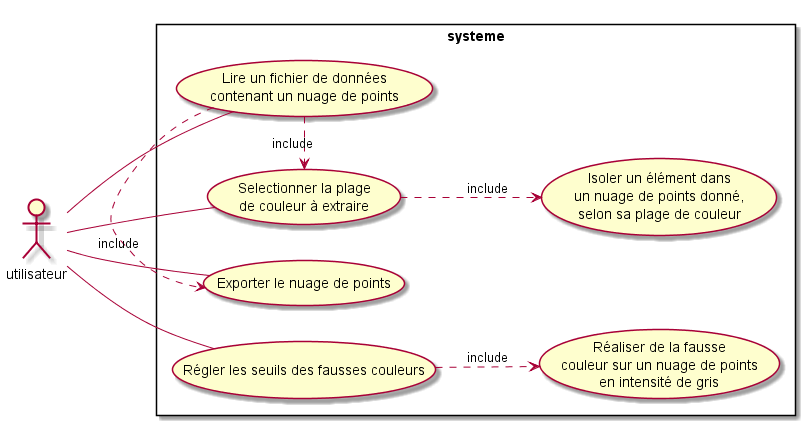
\includegraphics[scale=0.6]{img_diagrammes/use_cases.png}
\end{figure}

\break
\subsection*{User stories}

Afin de décrire précisément le déroulement des différents cas d'utilisation présentés, il convient de réaliser des "user stories".
Chaque "user story" correspond à un cas d'utilisation.
Pour chacun des cas on décrit le scénario nominal (si tout se déroule comme prévu), et les scénarios secondaires décrivant des comportements imprévus.
\begin{enumerate}
    \item \textbf{Lire un fichier de données contenant un nuage de points}

En tant qu'utilisateur du logiciel, je souhaite lire un fichier contenant un nuage de points afin d'avoir sa visualisation en 3D.

\textbf{Tests d'acceptation :}

\begin{enumerate}
    \item \textbf{Scénario 1}
Étant donné que je suis sur un terminal de commandes\\
Quand je lance le programme en renseignant un fichier de nuage de points en paramètre\\
Alors une fenêtre apparaît avec la visualisation du nuage en 3D.

    \item \textbf{Scénario 2}
Étant donné que je suis sur un terminal de commandes\\
Quand je lance le programme en renseignant un fichier de mauvais format\\
Alors un message d'erreur indiquant que le format de fichier ne correspond pas apparaît.

    \item \textbf{Scénario 3}
Étant donné que je suis sur un terminal de commandes\\
Quand je lance le programme en renseignant un fichier de nuage de points avec une mauvaise structure (XYZ + RGB + intensité)\\
Alors un message d'erreur indiquant que la structure du fichier ne correspond pas apparaît.

\end{enumerate}

    \item \textbf{Isoler un élément dans le nuage de points, selon sa plage de couleur}

En tant qu'utilisateur du logiciel, je souhaite isoler un élément dans le nuage de points afin d'afficher à l'écran uniquement l'élément voulu selon sa couleur.

\textbf{Tests d'acceptation :}

\begin{enumerate}
    \item \textbf{Scénario 1}

Étant donné que j'ai affiché un nuage de points via un fichier\\
Quand je clique sur l'option pour isoler un élément\\
Alors une interface avec un color picker apparaît\\
Quand je sélectionne une plage de couleur\\
Et que je clique sur le bouton de validation\\
Alors le nuage de points n'affiche uniquement que les points respectant la plage d'intensité de couleur.

\end{enumerate}
\item \textbf{Réaliser de la fausse couleur sur un nuage de points en intensité de gris}

En tant qu'utilisateur du logiciel, je souhaite faire ressortir des variations de gris du nuage en fausse couleur afin de mettre en lumière de nouveaux éléments et faciliter la compréhension.

\textbf{Tests d'acceptation :}

\begin{enumerate}
    \item \textbf{Scénario 1}

Étant donné que j'ai affiché un nuage de points via un fichier\\
Quand je clique sur l'option fausse couleur\\
Alors une interface avec un outil utilisateur apparaît\\
Quand je sélectionne l'intensité de gris à mettre en fausse couleur\\
Et que je choisis la couleur voulue\\
Et que je clique sur le bouton de validation\\
Alors le nuage de point s'affiche en fausse couleur.
\end{enumerate}

\item \textbf{Exporter le nuage de points}

En tant qu'utilisateur du logiciel, je souhaite enregistrer les modifications que j'ai effectué en exportant le nuage de points actuel sous la forme d'un fichier pouvant être ouvert dans un autre programme.

\textbf{Tests d'acceptation :}

\begin{enumerate}
    \item \textbf{Scénario 1}
Étant donné que j'ai affiché un nuage de points via un fichier et que je l'ai modifié\\
Quand je clique sur le bouton de sauvegarde\\
Alors une fenêtre apparaît proposant de choisir le formatage des données, c'est-à-dire l'ordre des colonnes\\
Aucun format n'est choisi par défaut\\
Je choisis l'ordre des colonnes qui me convient en le cochant\\
Je clique sur le bouton Appliquer\\
La fenêtre se ferme\\
Une nouvelle fenêtre demandant de choisir un emplacement dans l'explorateur de fichiers apparait\\
Je choisis une localisation dans l'explorateur de fichiers\\
Et je choisis un nom\\
J'appuie sur le bouton d'enregistrement\\
Le fichier est enregistré à l'emplacement sélectionné avec le nom choisi.

    \item \textbf{Scénario 2}
Étant donné que j'ai affiché un nuage de points via un fichier et que je l'ai modifié\\
Quand je clique sur le bouton de sauvegarde\\
Alors une fenêtre apparaît proposant de choisir le formatage des données, c'est-à-dire l'ordre des colonnes\\
Aucun format n'est choisi par défaut\\
Je choisis l'ordre des colonnes qui me convient en le cochant\\
Je clique sur le bouton Appliquer\\
La fenêtre se ferme\\
Une nouvelle fenêtre demandant de choisir un emplacement dans l'explorateur de fichiers apparait\\
Je choisis une localisation dans l'explorateur de fichiers\\
Et je choisis un nom invalide (avec des caractères interdits)\\
J'appuie sur le bouton d'enregistrement\\
Alors un message d'erreur indiquant que le nom choisi est invalide apparaît\\
Je peux modifier le nom du fichier.

    \item \textbf{Scénario 3}
Étant donné que j'ai affiché un nuage de points via un fichier et que je l'ai modifié\\
Quand je clique sur le bouton de sauvegarde\\
Alors une fenêtre apparaît proposant de choisir le formatage des données, c'est-à-dire l'ordre des colonnes\\
Aucun format n'est choisi par défaut\\
Je choisis l'ordre des colonnes qui me convient en le cochant\\
Je clique sur le bouton Appliquer\\
La fenêtre se ferme\\
Une nouvelle fenêtre demandant de choisir un emplacement dans l'explorateur de fichiers apparaît\\
Je choisis une localisation dans l'explorateur de fichiers\\
Et je choisis un nom correspondant à un fichier déjà existant\\
J'appuie sur le bouton d'enregistrement\\
Alors un message d'alerte indiquant qu'un fichier portant le même nom existe déjà apparaît, j'ai le choix d'écraser ou d'annuler\\
Je choisis d'écraser le fichier\\
Alors le fichier est enregistré à l'emplacement sélectionné avec le nom choisi, remplaçant le fichier existant.

\end{enumerate}
\end{enumerate}

Chaque User story va nous permettre de tester notre solution, afin de savoir si ce que nous allons développer va correspondre avec les attentes du client. Il faudra alors dérouler chaque scénario définit précédemment, et constater si la fonctionnalité développée respecte son ou ses scénarios de tests d'acceptation.

\section{Besoins non fonctionnels}

Cette section regroupe les différentes contraintes techniques ainsi que les besoins secondaires pris en compte.\\

\noindent\begin{tabu} to \textwidth {X[c]X[c3]}\toprule
\thead{Fonctions}&\thead{Commentaires}\\\toprule
Performances de l'ordinateur
& A cause des nuages de points, il est nécessaire d'avoir des ordinateurs un minimum performant. Cela veut donc impliquer le fait que le programme développé nécessitera aussi un ordinateur performant.\\\midrule
Fichiers en entrée
& L'utilisation du programme devra vérifier la conformité des scans que l'on nous fournira.\\\midrule
Langage utilisé
& Il n'y a aucun langage requis par le client. Nous utiliserons Python, un langage maîtrisé par toute l'équipe de développement et adapté à la manipulation de données telles que des nuages de points\\\bottomrule \\
\end{tabu}

Nous pouvons constater qu'il n'y a pas énormément de besoins non fonctionnels à prendre en compte pour ce projet. Néanmoins, d'autres besoins non fonctionnels n'ont peut-être pas encore été définis jusqu'à maintenant mais pourront apparaître au cours du projet.

\section{Evolution potentielle des besoins}

Les besoins énoncés ici concernent des fonctionnalités que le client voudrait ajouter sur un de leur logiciel déjà existant (ScanSap). À termes, il voudra donc les ajouter directement sur ce dernier, au lieu d'avoir une utilisation externe comme prévue dans le cadre de notre projet transversal.

Il y a donc déjà des fonctionnalités existantes, sur des logiciels tels que Cloud Compare, permettant de nous aider sur nos besoins fonctionnels (par exemple, la lecture d'un scan, la segmentation d'une zone, etc.). La majeur partie à développer ici sera la fausse couleur et l'isolation de points.

Il sera également possible que la réalisation des tâches soit plus rapide que prévue. Des nouveaux besoins pourront donc apparaître chez le client, afin d'améliorer les outils ou de développer des nouvelles fonctionnalités qui n'ont pas été abordées jusqu'ici.


\section{Limites du projet}

La correction des erreurs et artéfacts des fichiers fournis en entrée du programme ne fait pas partie du projet.
De même que la visualisation du nuage de points directement depuis le programme. Cette fonctionnalité est assurée par le logiciel de l'entreprise, plus performant. Cette fonctionnalité peut être présente, mais uniquement à des fins de test.

\section{Risques}

Au cours de la réalisation du projet, des risques peuvent apparaître. Ce sont des situations qu'il est possible d'identifier au préalable, et qui pourront être un obstacle potentiel au développement du projet. Il est nécessaire de les noter au maximum, en se basant sur les connaissances de la MOE et de la MOA. Les différents risques pour ce projet sont listés ci-dessous :
\begin{enumerate}
\item Incapacité à distinguer les éléments de façon efficace dus à des artéfacts ou manques d'informations sur une zone du nuage de points
\item Impact trop important du mouchetage sur la qualité de la segmentation.
\item Des points résiduels qui restent dans le nuage de points après filtrage (notamment à cause des artéfacts).
\item Panne du matériel de travail.
\end{enumerate}

\section{Plannings}

La planification du projet est importante, car elle va permettre de situer le projet dans le temps, où la durée ici sera d'une année. Nous aurons alors une meilleure estimation de la charge de travail du projet, et de planifier les tâches à effectuer. 

\subsection*{Planning général}

Ce planning ci-dessous sous un diagramme de Gantt, reste assez flou et ne sera probablement pas la réalisation exacte de ce projet, puisqu'il est encore difficile de savoir parfaitement la capacité de travail de chacun d'entre nous, et de la charge de travail de chacune des tâches.

\begin{figure} [!hbtp]
 \centering
    \caption{Diagramme de Gantt général - Tableau des tâches}
    \label{Diagramme de Gantt général - Tableau des tâches}
    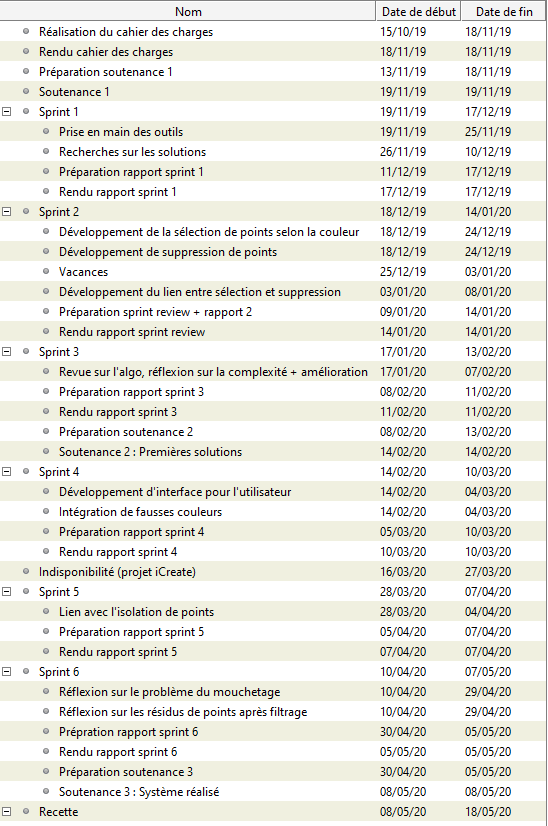
\includegraphics[scale=1,origin=c]{img_gantt/tableau_gantt_general.PNG}
\end{figure}
\break
\begin{figure} [!hbtp]
 \centering
    \caption{Diagramme de Gantt général - Affichage sur le temps}
    \label{Diagramme de Gantt général - Affichage sur le temps}
    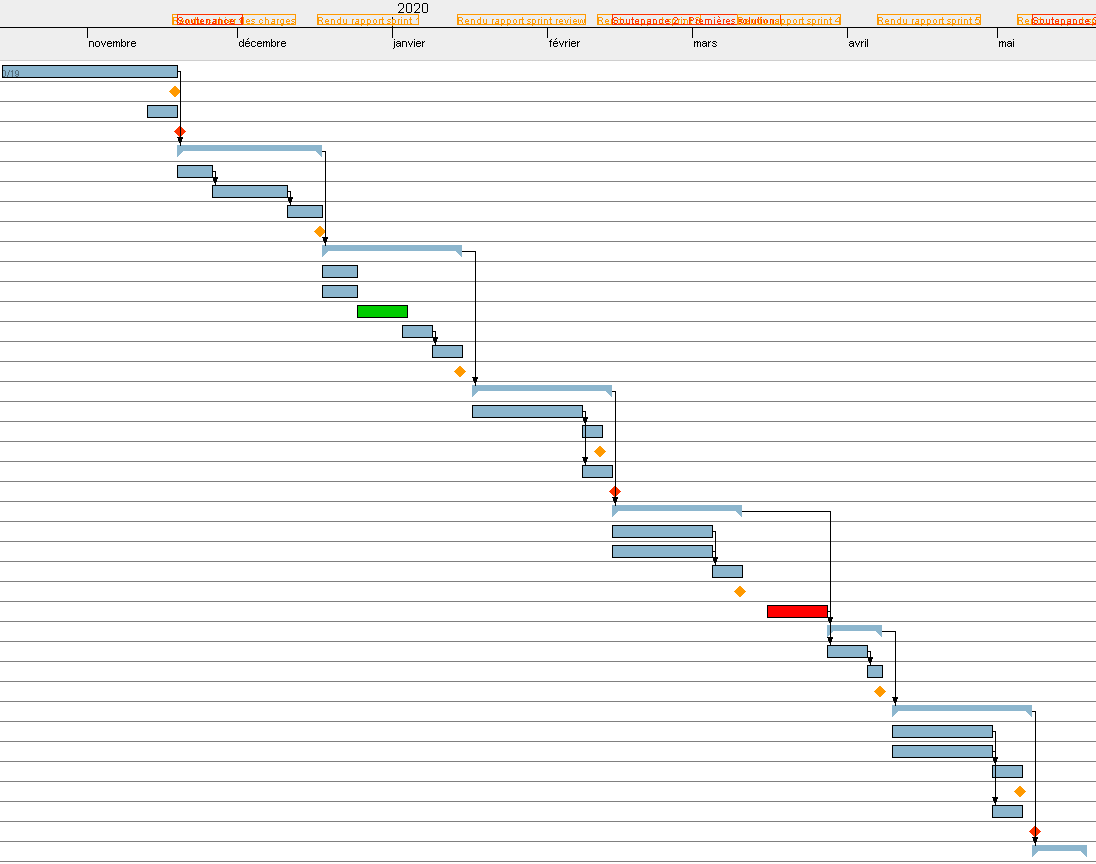
\includegraphics[scale=0.6, origin=c]{img_gantt/affichage_gantt_general.PNG}
\end{figure}

L'ensemble du Projet transversale se déroule de septembre à mi-mai. Et, il est jalonné par quatre grandes étapes :
\begin{enumerate}
\item De mi-septembre à mi-octobre : réalisation du Brief
\item De mi-octobre à mi-novembre : réalisation du Cahier des charges
\item De mi-novembre à début mai : développement itératif de la solution
\item Mi-mai : restitution du projet
\end{enumerate}

Ce diagramme de Gantt servira de fil directeur pour respecter les délais du projet. Il pourra potentiellement être amené à être modifié notamment au niveau de la description des itérations, puisqu'avec le fonctionnement du projet en méthodologie agile, les besoins pourront évoluer au fil du temps.

\subsection*{Planning détaillé itération 1}

Nous allons aussi présenter en détail la première itération. En effet, avant chaque nouvelle itération, il nous faudra estimer les sous-tâches à réaliser, au niveau du temps, mais aussi au niveau des ressources à allouer, c'est-à-dire quel étudiant ira travailler sur une certaine tâche.

\begin{figure} [!hbtp]
 \centering
    \caption{Diagramme de Gantt itération 1 - Tableau des tâches}
    \label{Diagramme de Gantt itération 1 - Tableau des tâches}
    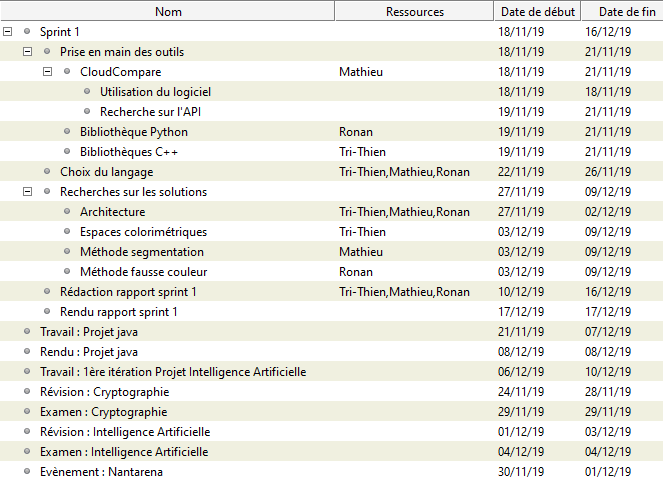
\includegraphics[scale=1,origin=c]{img_gantt/tableau_gantt_iteration1.PNG}
\end{figure}
\break
\begin{figure} [!hbtp]
 \centering
    \caption{Diagramme de Gantt itération 1 - Affichage sur le temps}
    \label{Diagramme de Gantt itération 1 - Affichage sur le temps}
    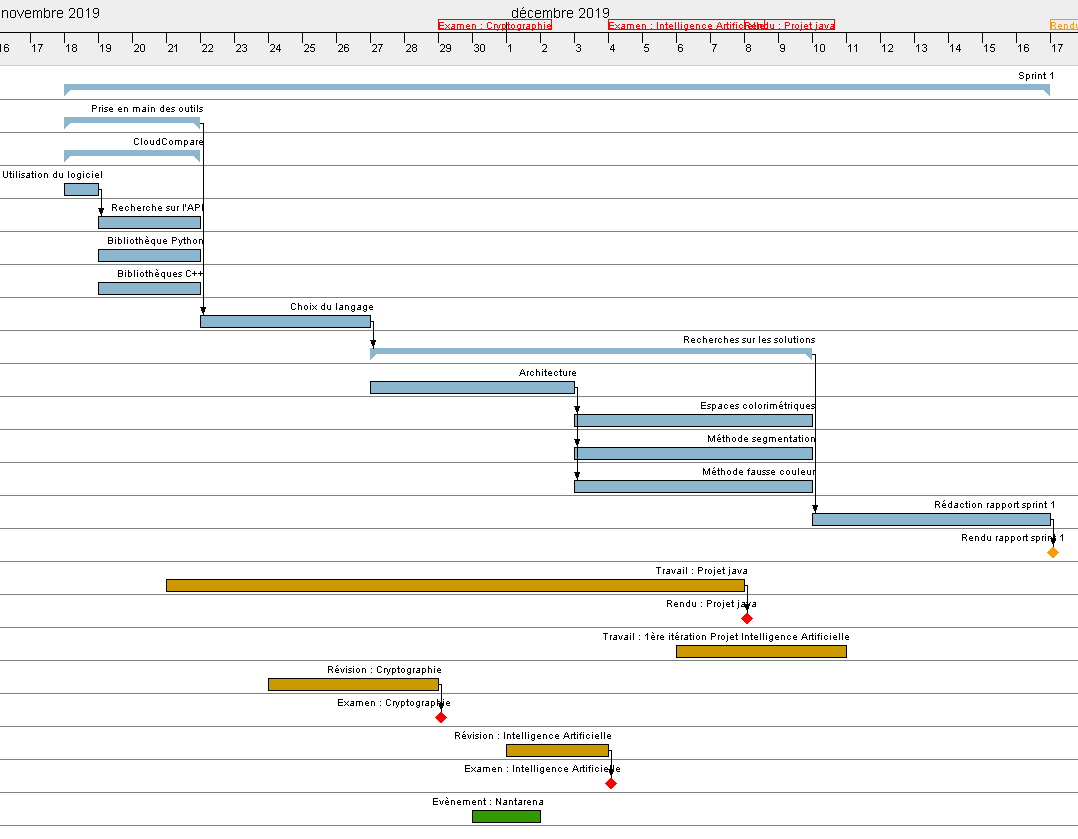
\includegraphics[scale=0.6, origin=c]{img_gantt/affichage_gantt_iteration1.PNG}
\end{figure}

La première itération sera consacrée à la recherche. Ainsi, nous réaliserons une recherche poussée sur les bibliothèques des langages qui sont le C++ et le Python, orientés sur la manipulation des nuages de points, afin de choisir le plus adéquat, et nous concentrer sur comment réaliser/répondre aux besoins de la segmentation et la fausse couleur. Pour ce faire, nous avons réparti au maximum les tâches pour qu'elles puissent être réaliser en parallèle.\\

Il faut aussi prendre en compte le fait qu'en tant qu'étudiant, nous aurons des contraintes externes au projet, qui nous limiterons sur le temps de travail sur celui-ci. Les tâches ici sont représentées de façon assez large, car elles prendront en compte ces contraintes, représentées en dessous sous d'autres couleurs.

\section{Gestion de projet}

Pour la bonne réalisation du projet en mode agile, certaines responsabilités devront être respectées du côté de la MOE et de la MOA.

La MOE se tient de fournir au client un suivi continu du projet. En effet, via les différents sprints qui seront réalisés, le client aura une visibilité sur l'évolution de la réalisation du projet, via des rapports, des prototypes et démonstrations. Ces évolutions seront disponibles à la fin de chaque sprint.

Quant à la MOA, elle se tient de garder un contact avec la MOE, et de respecter les rendez-vous convenus. De plus, elle pourra fournir des exemples de nuages de points permettant de réaliser des tests sur le projet. Si des conseils ou autres informations permettant le bon développement du projet peuvent être communiqués, la MOE pourra alors prendre contact avec la MOA pour se tenir informé.\\

\noindent\begin{tabularx}{\textwidth}{|X|X|X|}
    \hline
    \textbf{Date et signature du client :} & \textbf{Date et signature du chef de projet :} & \textbf{Date et signature du tuteur pédagogique}\\
    \hline
   \rule{0pt}{3cm} &
    &\\
    \hline

\end{tabularx}

\section{Connaissances utiles}

Cette section se remplira au fur et à mesure de l'avancement dans le projet.

\subsection*{Bibliothèques de manipulation de nuages de points}
Il existe de nombreuses bibliothèques permettant d'interagir avec les nuages de points. La majorité d'entre elles sont programmées en C++ et offrent souvent un support Python, qui semble être les deux langages phares du traitement de nuage de points.
Certaines bibliothèques se démarquent du lot et sont employés dans le cadre de projets ou d'activités de recherche.

C'est le cas de PCL (Point Cloud Library), une bibliothèque open source puissante proposant de nombreuses fonctionnalités allant de la segmentation à la reconnaissance en passant par la visualisation. Elle dispose également d'un module Python l'adaptant. Elle est distribuée sous licence BSD.

On peut également citer CloudViewer, une bibliothèque dont le champ d'application est plus large encore, puisqu'elle permet de gérer la 3D en général. Elle est disponible pour C++ et Python sous licence MIT.

PDAL (Point Data Abstraction Library), une bibliothèque moins connue, propose une manipulation des nuages de points au travers de "pipelines". Elle est développée en C++ sous licence BSD et propose également un support Python.

Bien que ces trois bibliothèques aient retenu notre attention, aucun choix pour l'une d'entre elle n'a encore été formulé. 

\newpage
\begin{thebibliography}{9}
\bibitem{cc} Présentation de Cloud Compare:
\url{https://www.danielgm.net/cc/}

\bibitem{3DList} Liste regroupant les principales bibliothèques 3D:
\url{https://github.com/openMVG/awesome_3DReconstruction_list#mesh-storage-processing}

\bibitem{PCL} Présentation de PCL:
\url{http://www.pointclouds.org/}

\bibitem{CloudViewer} Présentation de CloudViewer:
\url{http://www.open3d.org/}

\bibitem{PDAL} Présentation de PDAL:
\url{https://pdal.io/index.html}

\bibitem{seg} Punya Prasad Sapkota, \textit{Segmentation of Coloured Point Cloud Data}, 2008
\url{https://pdfs.semanticscholar.org/efdb/3ff43d5beffa3845e6434b580f775e2abf85.pdf}

\bibitem{seg1} Erzhuo Che, Jaehoon Jung, et Michael J. Olsen, \textit{Object Recognition, Segmentation, and Classification of Mobile Laser Scanning Point Clouds: A State of the Art Review}, 2019
\end{thebibliography}
\end{document}